\documentclass[12pt]{article}
\usepackage[margin=2.5cm]{geometry}
\usepackage{enumerate}
\usepackage{amsfonts}
\usepackage{amsmath}
\usepackage{fancyhdr}
\usepackage{amsmath}
\usepackage{amssymb}
\usepackage{amsthm}
\usepackage{mdframed}
\usepackage{graphicx}
\usepackage{subcaption}
\usepackage{adjustbox}
\usepackage{listings}
\usepackage{xcolor}
\usepackage{courier}
\usepackage[utf]{kotex}
\usepackage{hyperref}

\definecolor{codegreen}{rgb}{0,0.6,0}
\definecolor{codegray}{rgb}{0.5,0.5,0.5}
\definecolor{codepurple}{rgb}{0.58,0,0.82}
\definecolor{backcolour}{rgb}{0.95,0.95,0.92}

\lstdefinestyle{mystyle}{
    backgroundcolor=\color{backcolour},
    commentstyle=\color{codegreen},
    keywordstyle=\color{magenta},
    numberstyle=\tiny\color{codegray},
    stringstyle=\color{codepurple},
    basicstyle=\ttfamily\footnotesize,
    breakatwhitespace=false,
    breaklines=true,
    captionpos=b,
    keepspaces=true,
    numbers=left,
    numbersep=5pt,
    showspaces=false,
    showstringspaces=false,
    showtabs=false,
    tabsize=1
}

\lstset{style=mystyle}

\pagestyle{fancy}
\renewcommand{\headrulewidth}{0.4pt}
\lhead{CSC 369}
\rhead{Worksheet 6 Solution}

\begin{document}
\title{CSC 369 Worksheet 6 Solution}

\maketitle

\bigskip

\begin{enumerate}[1.]
    \item Done. See link \href{https://www.man7.org/linux/man-pages/man1/free.1.html}{here}
    \item

    First, I need to find out how much memory is in my system, and how much is free.

    Running the command \texttt{free -m}, we have

    \begin{center}
    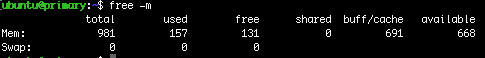
\includegraphics[width=0.8\linewidth]{images/worksheet_6_solution_1.png}
    \end{center}


    Using this information, I can write that the computer has

    \bigskip

    \begin{itemize}
        \item 981 MB of total memory
        \item 131 MB of free memory
    \end{itemize}

    \bigskip

    Second, I need to answer if these numbers match my intuition.

    \bigskip

    It does match my inution that free memory should be less than
    total memory.

    \bigskip

    \underline{\textbf{Notes}}

    \begin{itemize}
        \item I should ask professor the type of intution the author was expecting
        \item Installing Ubuntu Virtual Machine link: \href{https://multipass.run/}{here}
        \item Start virtual machine by typing command: \texttt{multipass start ubuntu-lts}
    \end{itemize}

    \item

    I need to write a little program \texttt{question\_3.c} (I will create this instead of
    \texttt{memory-user.c} for recording keeping purposes) that uses a certain amount of memory.

    \bigskip

    It's critera are:

    \begin{itemize}
        \item The program should take one command-line argument: the number of megabytes of memory it will use.
        \item The program should allocate an array.
        \item The program should constantly stream through the array, touching each entry.
        \item The program should do this indefinitely, or for a certain amount of time also specified in command line.
    \end{itemize}

    \bigskip

    For it's solution, please referr to \texttt{question\_3.c}
\end{enumerate}

\end{document}